\documentclass[a4paper]{article}
\usepackage{times}
\usepackage[utf8]{inputenc}
\usepackage{selinput}
\usepackage{upquote}
\usepackage[margin=2cm, rmargin=4cm, tmargin=3cm]{geometry}
\usepackage{tcolorbox}
\usepackage{xspace}
\usepackage[french]{babel}
\usepackage{url}
\usepackage{hyperref}
\usepackage{fontawesome5}
\usepackage{marginnote}
\usepackage{ulem}
\usepackage{tcolorbox}
\usepackage{graphicx}
%\usepackage[top=Bcm, bottom=Hcm, outer=Ccm, inner=Acm, heightrounded, marginparwidth=Ecm, marginparsep=Dcm]{geometry}


\newtcolorbox{Example}[1]{colback=white,left=20pt,colframe=slideblue,fonttitle=\bfseries,title=#1}
\newtcolorbox{Solutions}[1]{colback=white,left=20pt,colframe=green,fonttitle=\bfseries,title=#1}
\newtcolorbox{Conseils}[1]{colback=white,left=20pt,colframe=slideblue,fonttitle=\bfseries,title=#1}
\newtcolorbox{Warning}[1]{colback=white,left=20pt,colframe=warning,fonttitle=\bfseries,title=#1}

\setlength\parindent{0pt}

  %Exercice environment
  \newcounter{exercice}
  \newenvironment{Exercice}[1][]
  {
  \par
  \stepcounter{exercice}\textbf{Question \arabic{exercice}:} (\faClock \enskip \textit{#1})
  }
  {\bigskip}
  

% Title
\newcommand{\titre}{\begin{center}
  \section*{Algorithmes et Pensée Computationnelle}
\end{center}}
\newcommand{\cours}[1]
{\begin{center} 
  \textit{#1}\\
\end{center}
  }


\newcommand{\exemple}[1]{\newline~\textbf{Exemple :} #1}
%\newcommand{\attention}[1]{\newline\faExclamationTriangle~\textbf{Attention :} #1}

% Documentation url (escape \# in the TP document)
\newcommand{\documentation}[1]{\faBookOpen~Documentation : \href{#1}{#1}}

% Clef API
\newcommand{\apikey}[1]{\faKey~Clé API : \lstinline{#1}}
\newcommand{\apiendpoint}[1]{\faGlobe~Url de base de l'API \href{#1}{#1}}

%Listing Python style
\usepackage{color}
\definecolor{slideblue}{RGB}{33,131,189}
\definecolor{green}{RGB}{0,190,100}
\definecolor{blue}{RGB}{121,142,213}
\definecolor{grey}{RGB}{120,120,120}
\definecolor{warning}{RGB}{235,186,1}

\usepackage{listings}
\lstdefinelanguage{texte}{
    keywordstyle=\color{black},
    numbers=none,
    frame=none,
    literate=
           {é}{{\'e}}1
           {è}{{\`e}}1
           {ê}{{\^e}}1
           {à}{{\`a}}1
           {â}{{\^a}}1
           {ù}{{\`u}}1
           {ü}{{\"u}}1
           {î}{{\^i}}1
           {ï}{{\"i}}1
           {ë}{{\"e}}1
           {Ç}{{\,C}}1
           {ç}{{\,c}}1,
    columns=fullflexible,keepspaces,
	breaklines=true,
	breakatwhitespace=true,
}
\lstset{
    language=Python,
	basicstyle=\bfseries\footnotesize,
	breaklines=true,
	breakatwhitespace=true,
	commentstyle=\color{grey},
	stringstyle=\color{slideblue},
  keywordstyle=\color{slideblue},
	morekeywords={with, as, True, False, Float, join, None, main, argparse, self, sort, __eq__, __add__, __ne__, __radd__, __del__, __ge__, __gt__, split, os, endswith, is_file, scandir, @classmethod},
	deletekeywords={id},
	showspaces=false,
	showstringspaces=false,
	columns=fullflexible,keepspaces,
	literate=
           {é}{{\'e}}1
           {è}{{\`e}}1
           {ê}{{\^e}}1
           {à}{{\`a}}1
           {â}{{\^a}}1
           {ù}{{\`u}}1
           {ü}{{\"u}}1
           {î}{{\^i}}1
           {ï}{{\"i}}1
           {ë}{{\"e}}1
           {Ç}{{\,C}}1
           {ç}{{\,c}}1,
    numbers=left,
}

\newtcbox{\mybox}{nobeforeafter,colframe=white,colback=slideblue,boxrule=0.5pt,arc=1.5pt, boxsep=0pt,left=2pt,right=2pt,top=2pt,bottom=2pt,tcbox raise base}
\newcommand{\projet}{\mybox{\textcolor{white}{\small projet}}\xspace}
\newcommand{\optionnel}{\mybox{\textcolor{white}{\small Optionnel}}\xspace}
\newcommand{\advanced}{\mybox{\textcolor{white}{\small Pour aller plus loin}}\xspace}
\newcommand{\auto}{\mybox{\textcolor{white}{\small Auto-évaluation}}\xspace}


\usepackage{environ}
\newif\ifShowSolution
\NewEnviron{solution}{
  \ifShowSolution
	\begin{Solutions}{\faTerminal \enskip Solution}
		\BODY
	\end{Solutions}
  \fi}


  \usepackage{environ}
  \newif\ifShowConseil
  \NewEnviron{conseil}{
    \ifShowConseil
    \begin{Conseils}{\faLightbulb \quad Conseil}
      \BODY
    \end{Conseils}

    \fi}

    \usepackage{environ}
  \newif\ifShowWarning
  \NewEnviron{attention}{
    \ifShowWarning
    \begin{Warning}{\faExclamationTriangle \quad Attention}
      \BODY
    \end{Warning}

    \fi}
  

%\newcommand{\Conseil}[1]{\ifShowIndice\ \newline\faLightbulb[regular]~#1\fi}


\usepackage{array}
\usepackage{tabto}
\newcolumntype{C}[1]{>{\centering\let\newline\\\arraybackslash\hspace{0pt}}m{#1}}

\begin{document}

% Change the following values to true to show the solutions or/and the hints
\ShowSolutiontrue
\ShowConseiltrue
\titre
\cours{Algorithmes spatiaux}

Le but de cette séance est de comprendre la structure de données spatiales et d'implémenter quelques algorithmes d'indexation spatiale. Au terme de cette séance, l'étudiant sera en mesure d'utiliser quelques algorithmes spatiaux pour résoudre des problèmes de base de façon efficiente. \\

\section{Nearest-Neighbor}
Dans cette section, nous allons implémenter une recherche du plus proche voisin. Le but de cette méthode est de trouver le voisin le plus proche du point de départ en tenant compte de ce point de ``départ" et un ensemble de points. Nous allons implémenter cet algorithme et ensuite l'étendre à un algorithme des ``k plus proches voisins'' (recherche des k voisins les plus proches plutôt que du seul voisin le plus proche).\\
Nous vous recommandons de traiter les questions dans l'ordre.\\

\begin{Exercice}[5 minutes]\textbf{La fonction de distance : Python}\\

Pour implémenter notre recherche, nous avons besoin d'écrire une fonction permettant de calculer la distance euclidienne entre 2 points. Ecrivez une fonction qui permet de calculer la distance entre 2 points.\\

\begin{conseil}
    Soit 2 points en 2 dimensions $({x_1},{y_1})$ et $({x_2},{y_2})$, la distance euclidienne entre ces 2 points est donnée par : $\sqrt{(x_2-x_1)^2+(y_2-y_1)^2}$\\
    Vous pouvez définir un point comme étant un tuple de deux entiers. Exemple: \lstinline{point1=(4,5); point2=(1,3)}
\end{conseil}

\begin{solution}
   \lstinputlisting[language = python]{Question1_solution.py}
   Note : Vous auriez pu utiliser (...)**0.5 en lieu et place de la fonction math.sqrt(.)
\end{solution}
\end{Exercice}

\begin{Exercice}[10 minutes]\textbf{Nearest-neighbor search}\\

Implémentez la recherche du voisin le plus proche. L'algorithme fonctionne de la façon suivante :
\begin{enumerate}
    \item Traversez chaque point.
    \item Pour chaque point, calculez sa distance par rapport au point de départ.
    \item Retournez les coordonnées du point le plus proche.
\end{enumerate}
Votre fonction devra retourner les coordonnées (x,y) du point le plus proche ainsi que sa distance par rapport au point de départ.
    
\begin{conseil}
    Utilisez la fonction de distance de la question 1 et parcourez les points à l'aide d'une boucle \lstinline{for}. Si votre input est \lstinline{[[2,3],[5,6],[1,4],[2,4],[3,5]]} et que le point de départ est \lstinline{[4,4]}, alors l'output devra être ([3,5] 1.414).\\
    
    Note : Pour que votre programme fonctionne, écrivez votre algorithme du plus proche voisin dans le même programme que celui de la Question 1.
\end{conseil}
\begin{solution}
    % TODO: Dans le programme, faites appel à la fonction en lui passant des arguments.
    Note : Veillez à ajouter la fonction définie à l'exercice 1 pour que ce bout de code fonctionne.
    \lstinputlisting[language = python]{Question2_solution.py}
\end{solution}
\end{Exercice}
\begin{note}{Maeva}
    Ceci devrait être un exercice avancé
\end{note}
\begin{Exercice}[15 minutes]\textbf{K-nearest-neighbor search}\\

Améliorez l'algorithme créé précédemment afin qu'il puisse trouver les K plus proches voisins.\\

\begin{conseil}
Appliquez l'algorithme du plus proche voisin K-fois. À la fin de chaque itération retirez le voisin le plus proche de l'ensemble des points sur lequel l'algorithme s'applique. De cette façon, vous trouverez le second voisin le plus proche, le troisième, etc...\\

Votre fonction devra retourner une liste sous la forme :~$[[x_1,y_2, distance1],[x_2,y_2,distance2],...]$. Avec comme entrée [[2,3],[5,6],[1,4],[2,4],[3,5]], comme point de départ [4,4] et un nombre de voisins K=2, votre algorithme retournera : $[[3, 5, 1.4142], [2, 4, 2.0]]$.\\

Note : Pour que votre programme fonctionne, écrivez votre algorithme du plus proche voisin dans le même programme que celui des questions 1 et 2. Vous pouvez réutilisez le code des questions 1) et 2) pour cet exercice.
\end{conseil}

\begin{solution}
    Note : Veillez ajouter les fonctions des questions 1 et 2 pour que ce bout de code fonctionne.
    \lstinputlisting[language = python]{Question3_solution.py}
\end{solution}
\end{Exercice}
\newpage
\section{K-dimensional tree}

\begin{Exercice}[5 minutes]\textbf{KD-Tree, un échauffement : Papier}\\
Vous trouverez ci-dessous une liste de points numérotés de 1 à 10. Placez-les dans un KD-Tree et dessinez la séparation de l'espace qui en résulte.\\

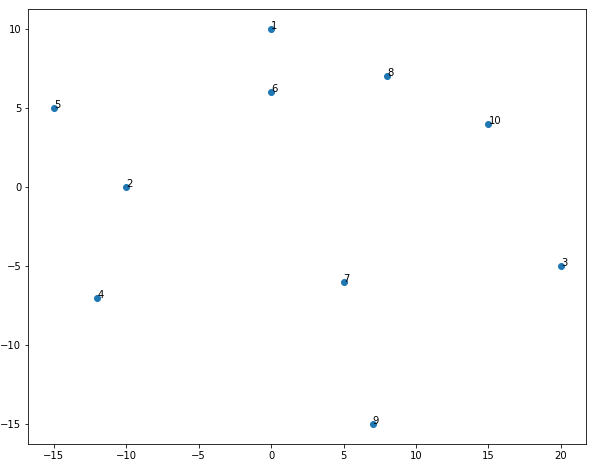
\includegraphics[]{KD_points.PNG}

\begin{conseil}
La première division se fait de façon verticale. Assurez-vous de bien insérer les points dans l'ordre (point 1, point 2, etc..). Les nœuds se situant au même niveau devraient diviser l'espace selon le même axe.
\end{conseil}
\begin{solution}
    Voici le KD-Tree correspondant :\\
    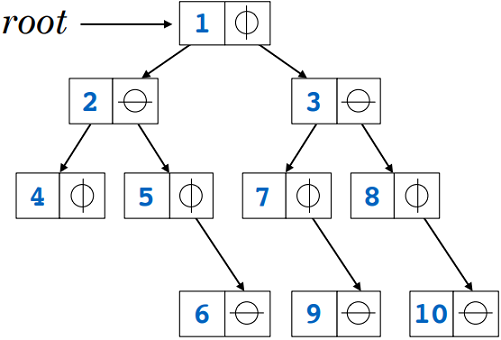
\includegraphics[]{Kd-tree.PNG}\\
    Et la division de l'espace qui en résulte :\\

    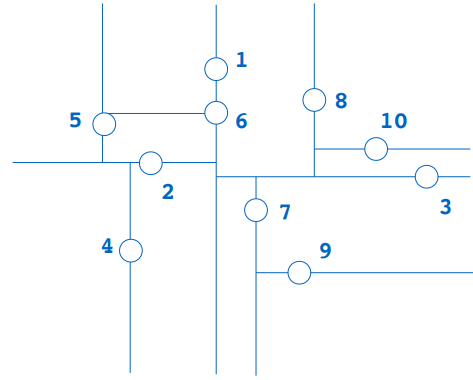
\includegraphics[scale=1]{DivisionEspace}
\end{solution}
\end{Exercice}

\newpage

\begin{Exercice}[15 minutes]\textbf{KD-Tree : Python}\\

L'objectif de cet exercice est d'écrire une fonction permettant d'ajouter un nœud à un KD-Tree. Les nœuds sont de la forme ((x,y), enfant à gauche, enfant à droite), x et y étant les coordonnées du nœud considéré. Complétez le code contenu dans le fichier \lstinline{Question5.py}.\\

\begin{conseil}
Voici le pseudo-code permettant d'ajouter un nœud à un KD-Tree :\\

ADD(node,point,cutaxis):\\
    \tabto{1cm}if node = NIL\\
        \tabto{2cm}node $\leftarrow$ Create-Node\\
        \tabto{2cm}node.point = point\\
        \tabto{2cm}return node\\
    \tabto{1cm}if point[cutaxis] $\leq$ node.point[cutaxis]\\
    \tabto{2cm} node.left = ADD(node.left, point, (cutaxis + 1) modulo k\\
    \tabto{1cm} else\\
    \tabto{2cm} node.right = ADD(node.right, point, (cutaxis+1) modulo k\\
    \tabto{1cm} return node\\
    
    Si votre réponse est correcte, le code de \lstinline{Question5.py} devrait afficher: [(0, 10), [(-10, 0), None, None], None].
\end{conseil}

\begin{solution}
    \lstinputlisting[language = Python]{Question5_solution.py}

    \underline{Commentaire \#1} : Si la coordonnée du point à ajouter est inférieure à celle du nœud selon l'axe de découpe en considération, alors le point doit se trouver dans le sous-arbre de gauche. Par convention, le nœud de gauche correspond dans la liste [(x,y), nœud de gauche, nœud de droite] à l'indice 1, par conséquent, on appelle la fonction de façon récursive pour ajouter le point, mais cette fois-ci en partant d'un cran plus bas dans l'arbre. Cela se répète jusqu'à ce qu'un ait atteint les feuilles et qu'un nouveau nœud doive être créé.

\end{solution}
\end{Exercice}

\newpage

\section{Quad-Tree}
\begin{Exercice}[10 minutes]\textbf{Une mise en train : Papier}\\

Encodez les images ci-dessous dans un Quad-Tree.\\

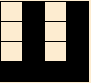
\includegraphics[]{Quad-Tree 1.PNG}\\
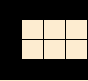
\includegraphics[]{Quad-Tree 2.PNG}

\begin{conseil}
    Pour réussir cet exercice, vous devez diviser chaque nœud en 4 sous-espaces de taille égale, et ce autant de fois que nécessaire. La branche la plus à gauche correspond au quadrant \lstinline{NW} puis en allant de gauche à droite : \lstinline{NE, SE, SW}.\\
    
    Votre arbre devrait avoir une profondeur de 2 et disposer de 16 feuilles.
\end{conseil}
\begin{solution}
    % TODO: Faire une vidéo pour expliquer le processus
    % TODO: À revoir
Image 1 :\\
    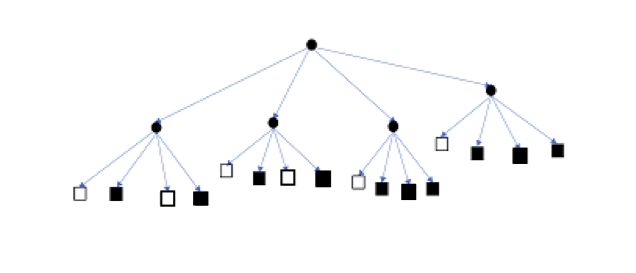
\includegraphics[]{Quad-Tree1Solution.PNG}\\
    
Image 2: \\
    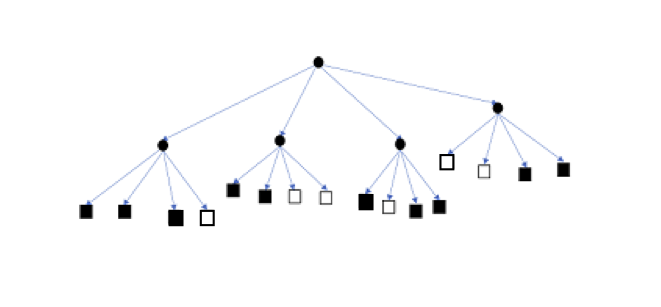
\includegraphics[]{Quad-Tree2Solution.PNG}\\\\
\end{solution}
\end{Exercice}

\begin{Exercice}[10 minutes]\textbf{Une mission capitale : Papier}\\

Récemment embauché par la CIA, vous êtes à la recherche d'un individu se cachant dans une des villes suivantes : Bleu, Orange, Noir, Gris, Vert et Jaune. Votre mission, si vous l'acceptez, est de créer un Quad-Tree qui vous permettra de géolocaliser le criminel de façon efficace. Vous trouverez ci-dessous une carte de villes. Créez le Quad-Tree et rétablissez la justice.\\


\begin{conseil}
    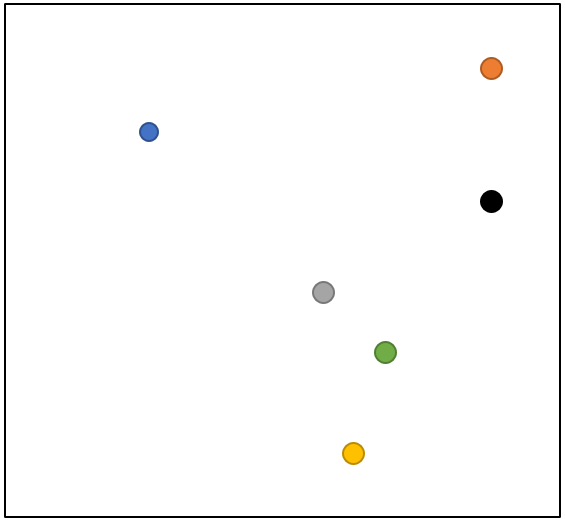
\includegraphics[scale=0.9]{Quad-Tree3.PNG}
    \\Commencez par diviser la carte de la ville de la façon adéquate puis construisez le graphe.\\
    
    \textbf{Remarque : }Les différentes branches de l'arbre n'auront pas toutes la même profondeur.
\end{conseil}
\begin{solution}
    Voici la division de la carte qui permet de construire le Quad-Tree :\\
    
    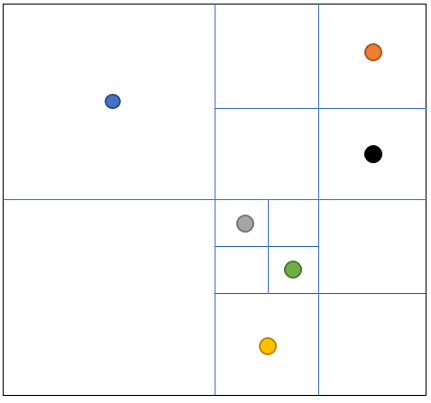
\includegraphics[]{Quad-Tree3Solution1.PNG}
    
    Le Quad-Tree qui en résulte :\\
    
    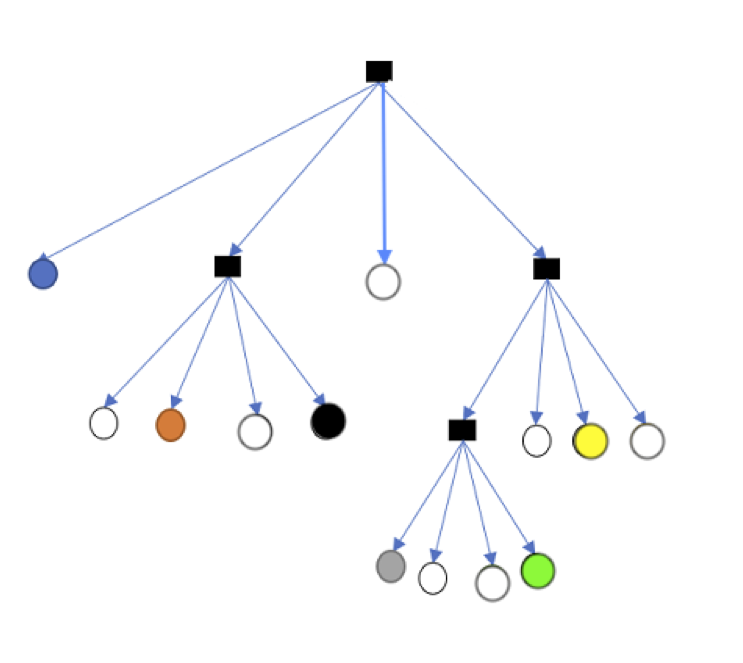
\includegraphics[]{Quad-Tree3Solution2.PNG}
    
    Note: Un rond blanc correspond à un quadrant vide.
    
\end{solution}
\end{Exercice}

\end{document}
